\documentclass[tikz]{standalone}
\usepackage{times}

\begin{document}

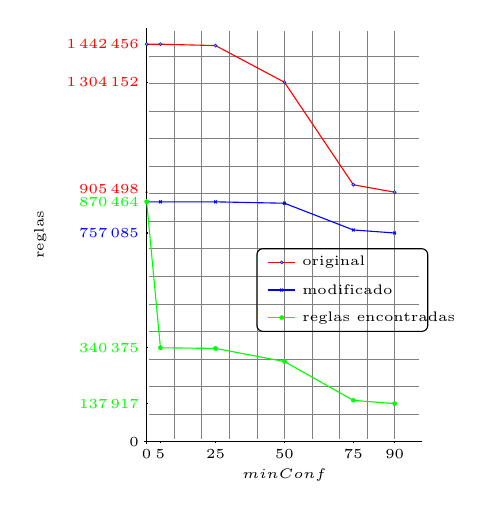
\begin{tikzpicture}[scale=.35]
	\tiny

   %ejes
   \draw (-0.1,0) -- (10,0);
   \draw (0,-0.1) -- (0,15);
   \draw[help lines,step=1cm] (0.1,0.1) grid (9.9,14.9);

   %marcas eje X
   \draw (5cm,-35pt) node {$minConf$};
   \draw (0cm,1pt) -- (0cm,-1pt) node[anchor=north] {0};
   \draw (.5cm,1pt) -- (.5cm,-1pt) node[anchor=north] {5};
   \draw (2.5cm,1pt) -- (2.5cm,-1pt) node[anchor=north] {25};
   \draw (5cm,1pt) -- (5cm,-1pt) node[anchor=north] {50};
   \draw (7.5cm,1pt) -- (7.5cm,-1pt) node[anchor=north] {75};
   \draw (9cm,1pt) -- (9cm,-1pt) node[anchor=north] {90};

   %marcas eje Y
   \draw (-110pt,7.5 cm) node[rotate=90] {reglas};
   \draw (1pt,0 cm) -- (-1pt,0 cm) node[anchor=east] {0};

   %Original
   \draw (1pt,9.05498 cm) -- (-1pt,9.05 cm) node[anchor=east,color=red,yshift=1pt] {905\,498};
   \draw (1pt,13.04 cm) -- (-1pt,13.04 cm) node[anchor=east,color=red] {1\,304\,152};
   \draw (1pt,14.42 cm) -- (-1pt,14.42 cm) node[anchor=east,color=red] {1\,442\,456};
   
   %Modificado
   \draw (1pt,7.57 cm) -- (-1pt,7.57 cm) node[anchor=east,color=blue] {757\,085};
   
   %Obtenidas
   \draw (1pt,8.70464 cm) -- (-1pt,8.70464 cm) node[anchor=east,color=green] {870\,464};
   \draw (1pt,3.40375 cm) -- (-1pt,3.40375 cm) node[anchor=east,color=green] {340\,375};
   \draw (1pt,1.37917 cm) -- (-1pt,1.37917 cm) node[anchor=east,color=green] {137\,917};
   
   %líneas
   \draw[color=red,style=solid] plot[mark=ball] coordinates {(0,14.42) (.5,14.42) (2.5,14.37) (5.0,13.04) (7.5,9.32) (9.0,9.05)};
   \draw[color=blue,style=solid] plot[mark=x] coordinates {(0,8.70) (.5,8.70) (2.5,8.70) (5.0,8.65) (7.5,7.68) (9.0,7.57)};
   \draw[color=green,style=solid] plot[mark=pentagon*] coordinates {(0,8.70464) (.5,3.40375) (2.5,3.38221) (5.0,2.90441) (7.5,1.49711) (9.0,1.37917)};
   
   %leyenda
   \draw[rounded corners=1ex] (4,4) rectangle (10.2,7);
   \draw (5.4,6.5) node[anchor=west](a) {original};
   \draw (5.4,5.5) node[anchor=west](b) {modificado};
   \draw (5.4,4.5) node[anchor=west](b) {reglas encontradas};
   \draw[color=red,style=solid] (4.4,6.5) -- (5.4,6.5) plot[mark=ball] coordinates {(4.9,6.5)};
   \draw[color=blue,style=solid] (4.4,5.5) -- (5.4,5.5) plot[mark=x] coordinates {(4.9,5.5)};
   \draw[color=green,style=solid] (4.4,4.5) -- (5.4,4.5) plot[mark=pentagon*] coordinates {(4.9,4.5)};
\end{tikzpicture}

\end{document}